% !BIB program = biber 
\documentclass{article}

%% Encoding
\usepackage[T1]{fontenc}
\usepackage[utf8]{inputenc}

%% Fonts
% Math fonts (fourier) with utopia (erewhon) text fonts
\usepackage{fourier, erewhon}
\usepackage{algorithm}
\usepackage[noend]{algpseudocode}
\usepackage{mathtools}

\DeclarePairedDelimiter\abs{\lvert}{\rvert}%
\DeclarePairedDelimiter\norm{\lVert}{\rVert}%
% Swap the definition of \abs* and \norm*, so that \abs
% and \norm resizes the size of the brackets, and the 
% starred version does not.
\makeatletter
\let\oldabs\abs
\def\abs{\@ifstar{\oldabs}{\oldabs*}}
%
\let\oldnorm\norm
\def\norm{\@ifstar{\oldnorm}{\oldnorm*}}
\makeatother

% Setup
% This package contains logos
 \usepackage[autoload]{adn}
 \setlogos[
 \textbf{MO433 --- Intro. to Unsupervised Machine Learning}\\%[5pt]
 \uppercase{Instituto de Computação --- UNICAMP}\\%[-7pt]
 ]%
 {IC3D}%
 {UNICAMP}

%% Transform section references
\makeatletter
\renewcommand*{\p@section}{\S\,}
\renewcommand*{\p@subsection}{\S\,}
\makeatother

%% Shorthands
\usepackage{xspace}
\makeatletter
\DeclareRobustCommand\onedot{\futurelet\@let@token\@onedot}
\def\@onedot{\ifx\@let@token.\else.\null\fi\xspace}

\def\eg{e.g\onedot} \def\Eg{E.g\onedot}
\def\ie{i.e\onedot} \def\Ie{I.e\onedot}
\def\cf{cf\onedot} \def\Cf{Cf\onedot}
\def\etc{etc\onedot} \def\vs{vs\onedot}
\def\wrt{w.r.t\onedot} \def\dof{d.o.f\onedot}
\def\etal{et al\onedot}
\makeatother

%%%
% Other packages start here (see the examples below)
%%

%% Figues
\usepackage{graphicx}
\graphicspath{{../output/}{./images/}}
\usepackage{caption}
\usepackage{subcaption}
\usepackage{array}
\usepackage{multirow}

%% References
% Use this section to embed your bibliography
% Instead of having a separate file, just place the bibtex entries here
\usepackage{filecontents}% create files
\begin{filecontents}{\jobname.bib}
@article{weng2018flow,
  title   = "Flow-based Deep Generative Models",
  author  = "Weng, Lilian",
  journal = "lilianweng.github.io/lil-log",
  year    = "2018",
  url     = "http://lilianweng.github.io/lil-log/2018/10/13/flow-based-deep-generative-models.html"
}

@article{ho2019flow++,
  title={Flow++: Improving flow-based generative models with variational dequantization and architecture design},
  author={Ho, Jonathan and Chen, Xi and Srinivas, Aravind and Duan, Yan and Abbeel, Pieter},
  journal={arXiv preprint arXiv:1902.00275},
  year={2019}
}

@misc{dinh2016density,
    title={Density estimation using Real NVP},
    author={Laurent Dinh and Jascha Sohl-Dickstein and Samy Bengio},
    year={2016},
    eprint={1605.08803},
    archivePrefix={arXiv},
    primaryClass={cs.LG}
}
\end{filecontents}
% Include bibliography file
\usepackage[
backend=biber, 
style=ieee, 
natbib=true,
]{biblatex}
\addbibresource{\jobname.bib}

%% Math
\usepackage{amsmath}

%% Enumerate
\usepackage{enumitem}

\begin{document}

% Put the topic of the assignment here
\title{Project 1}
% Put your name here 
\author{
Jo\~ao Victor da Silva Guerra,
Leonardo Alves de Melo,
and Marcos Felipe de Menezes Mota
\thanks{117410, 156188 and 211893. j117410@dac.unicamp.br, leonardo.alves.melo.1995@gmail.com., and marcos.mota@ic.unicamp.br}
}

\maketitle

\begin{abstract}

In this project, we attempt to reproduce an deep generative model, based on \textit{Flow++}, which is a flow-based model that explicitly learns the unconditional density function, $p(\boldsymbol{x})$, of real data. Flow models uses compositions of invertible functions as a way to circumvent the drawback of slow sample speed in other explicit density generative models (e.g autoregressive models). Thus, inference and sampling in flow models have similar complexity. The Flow++ architecture improves previous flow models with variational dequantization and more expressive architecture design. With these improvements, the model attain state-of-the-art performance within non-autoregressive models and similar performance to autoregressive models. This report shows our attempt to reproduce the Flow++ architecture using the CIFAR-10 dataset and the \textit{PyTorch} deep learning framework. We present the performance we attained with our implementation and samples generated from our trained architecture.  

\end{abstract}

\section{Introduction}

Exact likelihood models, such as autoregressive and non-autoregressive models, began to successfully model the probability density function of high dimensional data from real-world applications. 
Autoregressive models achieve state-of-the-art density estimation performance; however, this type of algorithm has a slow sampling procedure. The main reason is te sequential structure of autoregressive models where each output depends on the data observed in the past \cite{ho2019flow++, weng2018flow}.

Non-autoregressive flow-based models, denoted flow models, has an efficient sampling procedure, which comes from its structure composed by a sequence of invertible transformations ($f_i(x)$). As in autoregressive models, it explicitly learns the data distribution, using the loss function as the negative log-likelihood. However, flow models have shown worse results in density estimation benchmarks, such as CIFAR, ImageNet, CelebA, and so on.
An essential concern is the estimation of the latent variable ($z$), flow models carefully design transformations that make the estimation tractable, i. e., invertible transformation in the observed space.

In the next topic, we introduce the formal definitions of flow models and tractable flow functions ($f_i(x)$). After that, we present the \textit{Flow++} \cite{ho2019flow++}, a flow model that closes the performance gap between autogressive and non-autoregressive models, which design choices improves previous flow models.

\subsection{Flow Models}

A flow function is an invertible, stable, mapping between a data distribution $x \sim p_x$ and latent distribution $z \sim p_z$, where the latent distribution is typically a Gaussian \cite{dinh2016density}. Figure~\ref{fig:flow_latent} show an example of the effect of a flow function in a toy dataset. Since the inverse of a composition of functions is the composition of inverses of each component, we can define a flow model as composition of simpler invertible functions that does the mapping of data and latent variables.  

\begin{figure}
  \centering
  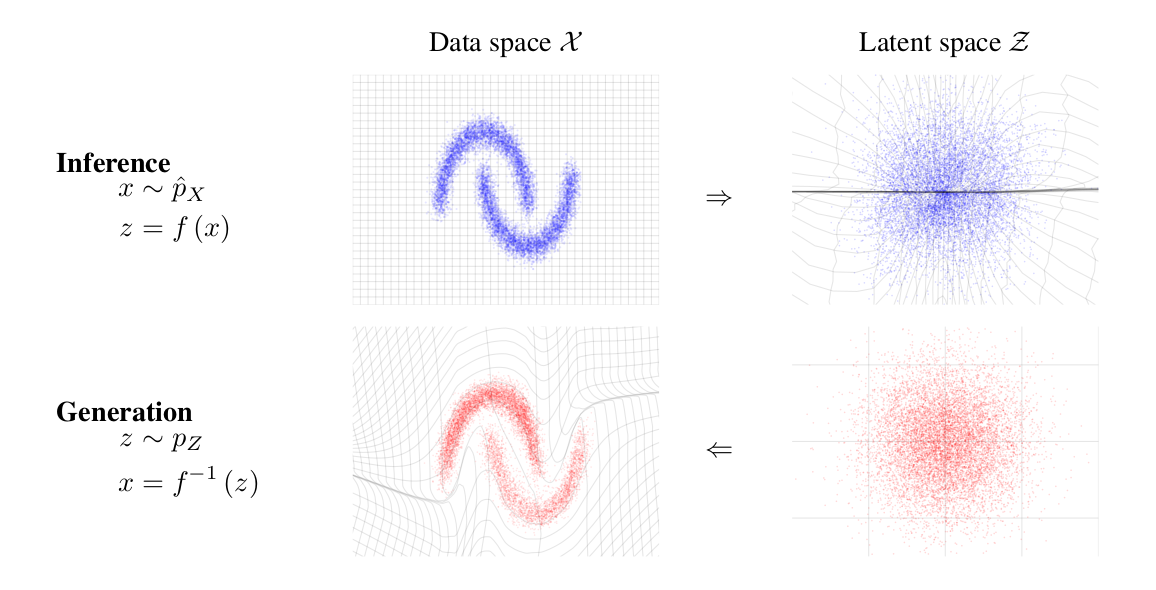
\includegraphics[width=0.65\linewidth]{images/flow_latent.png}
  \caption{Exemple of flow function \cite{dinh2016density}.}
  \label{fig:flow_latent}
\end{figure}

We define a function $f$ to be a flow model when the $f$ function maps observed data $x$ to a latent space in the form $z = f(x)$ and it is composed of $L$ functions of the form $f(x) = f_1 \circ f_2 \circ ... \circ f_L(x)$, such that each function $f_i$ is invertible and has a Jacobian. Using the change of variable equation, Equation~\ref{eq:chofvar}, and assuming that $z_i \sim \mathcal{N}(0,\boldsymbol{I})$ we can compute the maximum likelihood formula for flow models, Equation~\ref{eq:flow}:

\begin{equation}
  p_i(\boldsymbol{z}_i) = p_{i-1}(f_{i}^{-1}(\boldsymbol{z}_i))\abs{\text{det}\frac{\delta f_i^{-1}}{\delta \boldsymbol{z}_i}}
  \label{eq:chofvar}
\end{equation}

\begin{equation}
  \text{log}p(x) = \text{log}\mathcal{N}(f(x);0,I) + \sum^{L}_{i=1}\text{log}\abs{\text{det}\frac{\delta f_i}{\delta f_{i-1}}}
  \label{eq:flow}
\end{equation}

From Equation~\ref{eq:flow} and Figure~\ref{fig:coupling_flows} we can observe two features of flow models. First, the coupling of multiple base function define the expressivity of the density function learnt, so more complex coupling allows a more general task model. Second, the tractability of the maximum likelihood estimation depends on the computation of the model's Jacobian determinant. Therefore, one of the main tasks to design a new flow model is stablish a set of expressive function that has an easy to compute determinant.   

\begin{figure}
  \centering
  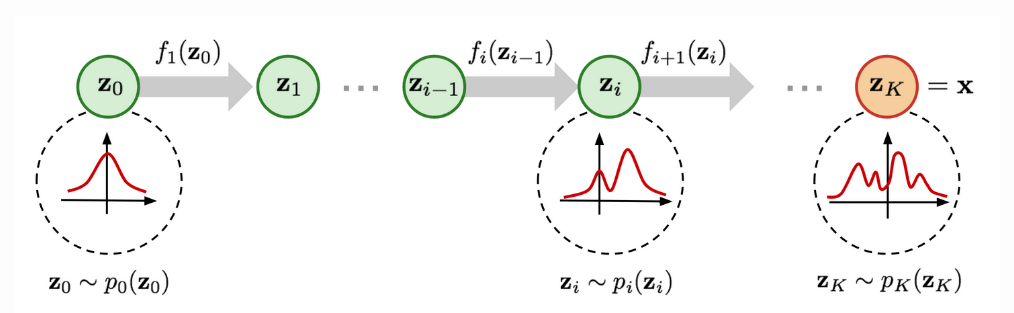
\includegraphics[width=0.7\linewidth]{images/flows_coupling.png}
  \caption{Coupling of function defining a complex flow model \cite{weng2018flow}.}
  \label{fig:coupling_flows}
\end{figure}


One solution to tractability in flow models is to use the fact that the determinant of diagonal or triangular matrices is the product of its diagonal terms. The most common choice of function for flow models is called \textit{affine coupling layer}. The coupling function and its Jacobian are defined below:
$$
\left\{\begin{matrix}
\mathbf{y}_{i:d}   = \mathbf{x}_{i:d}\\  
\mathbf{y}_{d+1:D} = \mathbf{x}_{d+1:D} \: \odot \mathrm{exp}(s(\mathbf{x}_{1:d})) + t(\mathbf{x}_{1:d}) 
\end{matrix}\right.
$$

$$
\textbf{J} = \begin{bmatrix}
\mathbb{I}_d & \textbf{0}_{d\times(D-d)}\\ 
\frac{\partial\textbf{y}_{d+1:D}}{\partial\textbf{x}_{1:d}}& \textrm{diag}(\textrm{exp}(s(\textbf{x}_{1:d}))) 
\end{bmatrix}
$$

This function has a Jacobian that is a triangular matrix, therefore it is easy to compute. Also, since the functions $s$ and $t$ are not involved in the Jacobian derivate they can be arbitrary complex function, thus can be implemented as neural networks. As we see in the next subsection Flow++ define more a more complex function set and other design improvements.

\subsection{Flow++}

\textit{Flow++} is a model that tries to improve previous flow models in three aspects: uniform dequantization is suboptimal, commonly used affine coupling flows are not expressive enough, and convolutional layers used withing the model can be more powerful. 

Dequantization is the process to convert a discrete data distribution into a continuos one. Previous models use uniform dequatization that adds noise drawn from $\text{Uniform}[0, 1)$ to the discrete data. However, such approach is not natural for neural networks. Thus, \textit{Flow++} relax the restriction of the noise coming from a uniform distribution and introduce a dequantization noise distribution $q(\boldsymbol{u})|x$, treating $q$ as an approximate posterior it is possible to establish a variational lower bound in the fashion of VAEs. The original paper report variational dequantization as the model that change that better improve Flow++ as generative model \cite{ho2019flow++}.

The second improvement of Flow++ is the use of a mixture os logistic functions as the flow function. The affine coupling that is used in other model is simple to compute and expressive, however, because of its linear structure, it has more problem in leaning non-linear features. Flow++ uses a CDF flow with mixture of logistic functions as we seen in Equation~\ref{eq:logi_coupling}. It has the same look of affine coupling but adds a logistic transformation on top. The Jacobian of the logistic CDF flow has the same structure of affine coupling, but involves calculating the probability density function of logistic mixtures which it is not computational difficult task. 

\begin{equation}\label{eq:logi_coupling}
\left\{\begin{matrix}
\textbf{y}_1 &= \textbf{x}_1 \\ 
\textbf{y}_2 &= \sigma^{-1}(\textrm{MixLogCDF}(\textbf{x}_2;\pi_{\theta}(\textbf{x}_1),\mu_{\theta}(\textbf{x}_1),\textbf{s}_{\theta}(\textbf{x}_1)))
\end{matrix}\right.
\end{equation}

where 
  $$\textrm{MixLogCDF}(x;\pi, \mu, \textbf{s}) := \sum_{i=1}^{K}\pi_i\sigma((x - \mu_i).\textrm{exp}(-s_i))$$

The third novelty in the Flow++ model is the use of self-attention with residual networks (ResNets). The use of residual networks with 1x1 convolutional layer was used in other models (e.g Glow), but stacking self-attention produce more powerful estimation. The sketch of the residual block for the Flow++ residual network is shown below:  

\begin{align*} \label{eq:res_block}
  \textrm{Conv} &= \textrm{Input} \rightarrow  \textrm{Nonlinearity} \rightarrow \textrm{Conv}_{3\times 3} \rightarrow \textrm{Nonlinearity} \rightarrow \textrm{Gate} \\
  \textrm{Attn} &= \textrm{Input} \rightarrow \textrm{Conv}_{1\times 1} \rightarrow \textrm{MultiHeadSelfAttention} \rightarrow \textrm{Gate}
\end{align*} 

\section{Dataset}

In our experiments, we used the CIFAR-10 dataset, which consists of 60000 images with 32x32 RGB pixels, totalizing 3072 features. The dataset contains 10 classes, with 5000 images for training set and 1000 images for test set for each class, some examples which can be seen in Figure \ref{fig:cifar}. 

\begin{figure}
  \centering
  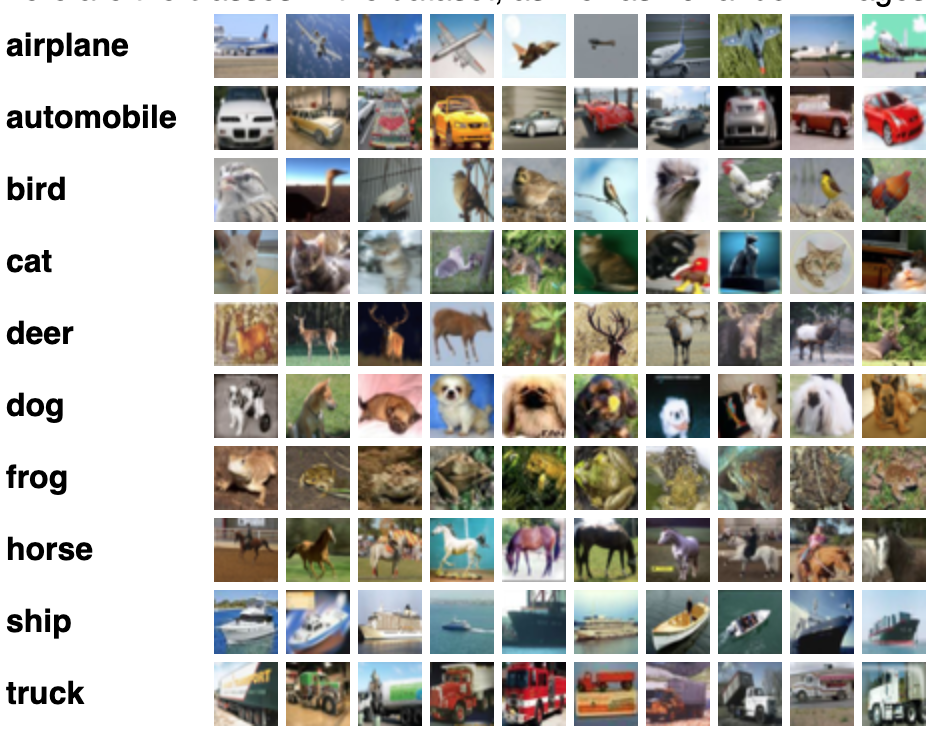
\includegraphics[width=0.8\linewidth]{cifar.png}
  \caption{Examples of CIFAR-10 classes.}
  \label{fig:cifar}
\end{figure}

For this project, we have trained our models for the entirely CIFAR-10 dataset and also for a subset containing only the labels described as \emph{dog}, that represents 6000 images of dogs, which can be seen in Figure \ref{fig:dogDatasetamples}. 

\begin{figure}
  \centering
  \includegraphics[width=0.8\linewidth]{dogs_cifar_trainset.png}
  \caption{Examples of dog images in CIFAR-10.}
  \label{fig:dogDatasetamples}
\end{figure}

\section{Implementation}

Considering that Flow++ is mostly a set of improvements over the RealNVP, our approach was first implementing a RealNVP algorithm to then adding the new components. Due to complexity implementation of this components, we simplified the algorithm to be executable with \emph{uniform dequantization} and simplified coupling of flows.

Our architecture code is divided in three main components \texttt{CouplingLayers}, \texttt{ResNet} and \texttt{Flow}. \texttt{ResNet} class define the convolutional network that will approximate the functions used inside the coupling flow layer, thus a stack of residual blocks containing the convolutions specified by the Flow++ model and batch normalization. \texttt{CouplingLayers} uses the \texttt{ResNet} together with the operation of coupling flows as explained in the Introduction. Also, \texttt{CouplingLayers} performs the coupling operations following the checkboard and channel-wise masks used in RealNVP \cite{dinh2016density} and Flow++ \cite{ho2019flow++}. At last, the \texttt{Flow} class setup the number of function in the coupling and the optmization of the flow for CIFAR-10 dataset with architecture forward step and loss function (NLL and conversion to bits/dim). All the variables in these classes are optmized using PyTorch Autograd methodology. 

For our experiments, we use a 4 residual blocks with 32 hidden feature maps for the first coupling layers with checkboard masking. We optimized the negative log-likelihood with ADAM optimizer with a fixed learning rate (1e-3 for CIFAR-10 and 1e-5 for dogs CIFAR-10 subset).

\section{Experiments}

We created two models, one for the entirely CIFAR-10 dataset, and the other for the dogs dataset. For the first one, we trained 30 epochs for the training and test set, and then generated 25 samples of the last epoch trained model. For the second one, we trained 50 epochs for both training and test set, and again generated 25 dogs samples for the last trained model.

\section{Results}

\subsection{Loss}

The decrease of the loss function in both training and test set for CIFAR-10 are shown in Figure \ref{fig:cifarLoss}. We noted that the negative log-likelihood loss decreases, but only in training set it smooth decrease until reach an seemingly stable state, showing that the algorithm converged. However, in the test set, the loss function starts diverging, being necessary to remove some outliers to be possible to see the its decrease. 

Now, the loss function of dogs dataset are shown in Figure \ref{fig:dogsLoss}. We notice that the loss function decreases in the training and test sets, but the test set shows more instability compared to the training set.

\begin{figure}
  \begin{subfigure}[t]{0.49\textwidth}
    \centering
    \includegraphics[width=\linewidth]{cifar/train_loss.png}
    \caption{Training set.}
    \label{fig:cifarTrainLoss}
  \end{subfigure}
  \hfill
  \begin{subfigure}[t]{0.49\textwidth}
    \centering
    \includegraphics[width=\linewidth]{cifar/test_loss.png}
    \caption{Test set.}
    \label{fig:cifarTestLoss}
  \end{subfigure}
  \caption{Loss function for CIFAR-10 dataset.}
  \label{fig:cifarLoss}
\end{figure}

\begin{figure}
  \begin{subfigure}[t]{0.49\textwidth}
    \centering
    \includegraphics[width=\linewidth]{dogs_cifar/train_loss.png}
    \caption{Training set.}
    \label{fig:dogsTrainLoss}
  \end{subfigure}
  \hfill
  \begin{subfigure}[t]{0.49\textwidth}
    \centering
    \includegraphics[width=\linewidth]{dogs_cifar/test_loss.png}
    \caption{Test set.}
    \label{fig:dogsTestLoss}
  \end{subfigure}
  \caption{Loss function for dogs CIFAR-10 subset.}
  \label{fig:dogsLoss}
\end{figure}

\subsection{Bits per Dimension}

The bits per dimension for the training and test sets of CIFAR-10 dataset are decreasing, as shown in Figure \ref{fig:cifarBpd}. At the last epoch, the test set has an bits per dimension of 7.07, which is greater than the values of RealNVP and Flow++ \cite{ho2019flow++}, respectively 3.49 and 3.08 over the CIFAR-10 dataset. For the dogs CIFAR-10 dataset, the bits per dimension, shown in Figure \ref{fig:dogsBpd}, are also high in the test set, reaching 6.41 at the last epoch. However, the bits per dimension in the training set stably descreases, which indicates a convergence of the network parameters.

The curve of bits per dimension has the exact same behaviour as the curve of loss function, because the second is the division of the fisrt by a constant (\ie number of dimensions). However, the bits per dimension could be used to compare data of different dimensions, such as CIFAR-10 and ImageNet 64x64, in exact likelihood models.

\begin{figure}
  \begin{subfigure}[t]{0.49\textwidth}
    \centering
    \includegraphics[width=\linewidth]{cifar/train_bpd.png}
    \caption{Training set.}
    \label{fig:cifarTrainBpd}
  \end{subfigure}
  \hfill
  \begin{subfigure}[t]{0.49\textwidth}
    \centering
    \includegraphics[width=\linewidth]{cifar/test_bpd.png}
    \caption{Test set.}
    \label{fig:cifarTestBpd}
  \end{subfigure}
  \caption{Bits per dimension for CIFAR-10.}
  \label{fig:cifarBpd}
\end{figure}

\begin{figure}
  \begin{subfigure}[t]{0.49\textwidth}
    \centering
    \includegraphics[width=\linewidth]{dogs_cifar/train_bpd.png}
    \caption{Training set.}
    \label{fig:dogsTrainBpd}
  \end{subfigure}
  \hfill
  \begin{subfigure}[t]{0.49\textwidth}
    \centering
    \includegraphics[width=\linewidth]{dogs_cifar/test_bpd.png}
    \caption{Test set.}
    \label{fig:dogsTestBpd}
  \end{subfigure}
  \caption{Bits per dimension for dogs CIFAR-10 subset.}
  \label{fig:dogsBpd}
\end{figure}

\subsection{Samples}

All samples are created with the network parameters from the last epoch of the training process. The samples are generated by inserting a random value of $z$ in reverse on our flow model. Hence, we show 25 samples of the network trained for CIFAR-10 and for dogs CIFAR-10 subset in Figure~\ref{fig:netSample} and \ref{fig:dogsNetSample}, respectively. For the CIFAR-10, we note that some configuration of colors and shapes are similar to animals, objects and natural settings. Further, for the dogs subset, we obserbed some shape and colors that poorly resembles a dog, showing that our model learned representations from the data. Taken together, our model could be learing some type of basic representation of the images that we provided, in which shows some hidden patterns of the data.


\begin{figure}
  \centering
  \includegraphics[width=\linewidth]{cifar/pre_trained_cifar.png}
  \caption{25 images sampled from the network for CIFAR-10.}
  \label{fig:netSample}
\end{figure}

\begin{figure}
  \centering
  \includegraphics[width=\linewidth]{dogs_cifar/pre_trained_dogs_cifar.png}
  \caption{25 images sampled from the network for dogs subset.}
  \label{fig:dogsNetSample}
\end{figure}

\section{Discussion}

The differences between our implementation and Flow++ have been responsible for the greater losses and bits per dimension for the CIFAR-10 dataset (dogs subset could not be compared); however, even with this differences, we got a nice set of samples, showing shapes and colors corresponding to the labels. For the dogs CIFAR-10 subset, the results seems more acceptable due to the stable behaviour of the loss function in the training and test set, which also yield nice samples with shapes and colors similar to dogs images. Taken together the test set loss of both dataset, the instability shown in the CIFAR-10 could be related to different learning rates, but a better tunning of the non-learnable parameters could led to a more stable behaviour.

The implementation of some network components, such as the ones described in Section 1.2, could led us to better results in density estimation performance (loss and bits per dimension). For example, an non-described implementation that would improve our results would be a dynamic learning rate, that could avoid reaching those outliers (\ie instability). Further, with access to powerful equipments, such as GPUs, our coding procedure would be better, we would reduce our trial and error time and we could test different approaches in much less time, including more Flow++ components. 

\section{Conclusion}

The attempt to reproduce a state-of-the-art generative model was an important step to bridge the gap between the theory behind these models and their implementation. Most of the team has little or no experience working with neural networks, thus the effort to reproduce the paper was really challenging. Besides that, we were able to generate sample from the model that present visual features of the data used to train the model. A major setback was the lack of equipment, like powerful GPUs to accelerate the training and run more epochs. If we had this type of equipment, we could have tested more components without losing a day for a training error, which would improve our trial and error capability. 

\printbibliography

\end{document}